\documentclass[11pt,a4paper]{article}
\usepackage[utf8]{inputenc}
\usepackage[T1]{fontenc}
\usepackage[english]{babel}
\usepackage{hyperref}
\usepackage{amsmath}
\usepackage{amsfonts, amsthm, bm}
\usepackage{mathrsfs}
\usepackage{graphicx}
\usepackage{amsthm}
\usepackage{newlfont}
\usepackage{color}
\usepackage{natbib}
\usepackage{float}
\usepackage{textcomp}


\textwidth=450pt\oddsidemargin=0pt

\renewcommand{\baselinestretch}{1,2}
\title{\Huge{\textbf{Study on Overfitting}} \\ 
                \vspace{5mm}
                \large{A review on Overfitting in Deep Learning convolutional models}}
\author{Mattia Ceccarelli}
\date{June 2020}

\begin{document}
\maketitle

The project aim is to study how overfitting can represent a problem in common data analisys tasks and how to detect and avoid it in Deep Learning Applications.

The datasets used over the whole study are \textit{MNIST-784}, composed of $70.000$, $28 x 28$ grey-scale images containing hand-written digits; and \textit{CIFAR-100}, composed of $60.000$, $32 x 32$ colored images comprehensive of $100$ classes of objects.

The study will also focus on how overfitting is influenced by the numbers of parameters.

All the data obtained in the case of Deep Learning models are obtained by using the famous python library Tensorflow \cite{tf} 

\section*{Overfitting in data analysis}

In the context of data analysis overfitting is a common problem that arises from different factor. 
The main cause of overfitting is noise: indeed, by definition, an analytical or statistical model is "overfitted" when the outcome of the algorithm is overly affected by the noise in the data, which means the model begin to describe the random error in the data rather that the relationship between variables.

This ordinary but important flaw of machine learning and deep learning model brings a series of consequences that have as a secondary effect to reduce the effectiveness of the model, in particular in data it has never seen before: this phenomenon is called lack of Generalizations capabilities.

An example of overfitting in analytical method is shown in figure \ref{polyfit} found when using a simple polynomial fit on randomly generated data from $f(x) = 5 * sin(x * 9 / 10) + \nu$ where $\nu$ is a normally distributed random variable with $\mu = 0$ and $\sigma = 1$. The results obtained in the case of high order polynomial can be considered as a form of overfitting since the model tries to exactly fit every random  point.    

\begin{figure}[H]

 \centering
 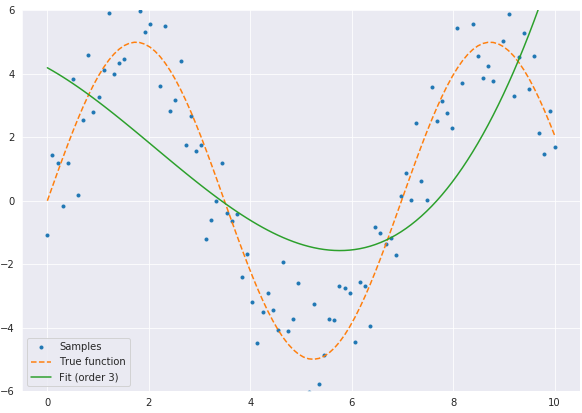
\includegraphics[scale=0.35]{../images/fit_nlinear_order3.png}
 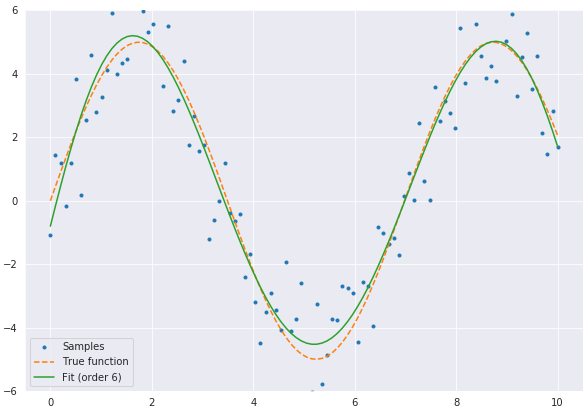
\includegraphics[scale=0.35]{../images/fit_nlinear_order6.png} \\
 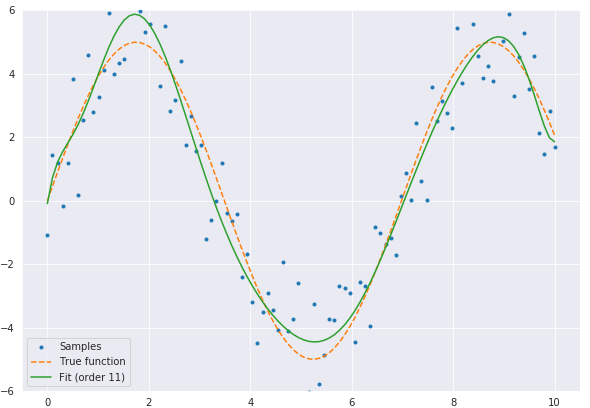
\includegraphics[scale=0.35]{../images/fit_nlinear_order11.png}
 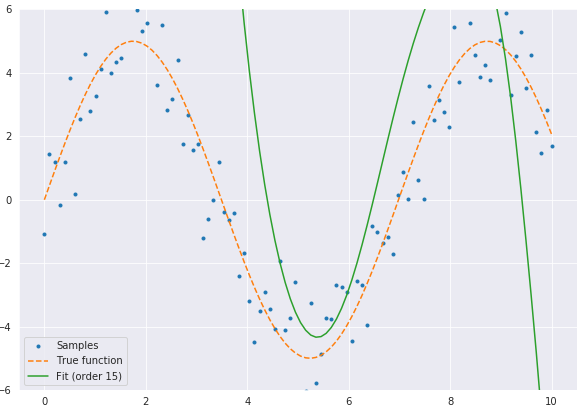
\includegraphics[scale=0.35]{../images/fit_nlinear_order15.png}
 \caption{\textit{The image shows in order from left to right and from up to down: underfitting of polynomial with order 3, best fit with polynomial of order 6, and overfitting with polynomial of order 11 and 15}}  
 \label{polyfit}
 
\end{figure}


Given the fact that noise can't be removed from data a priori, many different techniques has been developed to avoid overfitting. 
The most widely used is the simple divion between training data and test data, which allow more control over the performances of the models. Figure \ref{scheme} shows some variation of the same concept: keep train and test data separated.
This greatly reduce the risk of overfitting and the introduction of Validation sets helps with the fine-tuning of hyper-parameters. 
The advantages come at the cost of computational efficency.

\begin{figure}[H]

 \centering
 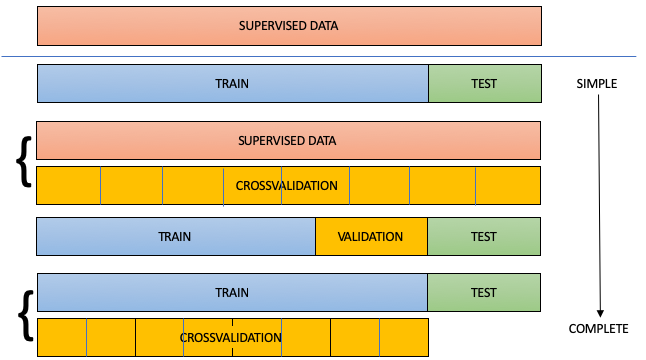
\includegraphics[scale=0.5]{../images/test_train_process.png}
 \caption{\textit{The image show the most common practices in machine learning application to maintain top generalization performances.}}  
 \label{scheme}
 
\end{figure}


Other causes for overfitting may come from the dataset: 

\begin{itemize}
 \item [-] individuals in the test set can have bad values in the predicting attributes
           and/or in the class label
 \item [-] Lack of representative instances some situations of the real world can be underrepresented, or not represented at all, in the training set. This situation is quite common.
\end{itemize}

As a rule, a good hypothesis has low generalization error i.e. it works well on examples different from those used in training.

\section*{Overfitting in Deep Learning}

In deep learning, overfitting is essentially threated the same as for other machine learning metods. 
It's easy to see how overfitting can appear in simple applications: in figure \ref{cifar-overfit-loss} is shown the charateristic trend of the loss in a overfitting model. 
In this case, the Gradient Descent is performed on the categorical crossentropy loss, defined as : 

\begin{equation}
  CE = -\sum_{i=1}^{classes} t_i log(x_i)
\end{equation}

Where $t_i$ is the true label of the input, while $x_i$ is the predicted label of the input.
As shown in the graph below, it is clear how, if not monitored, overfitting can and does lead to contradictory results (very good on training set, very bad on test set). 

\begin{figure}[H]
 \centering
 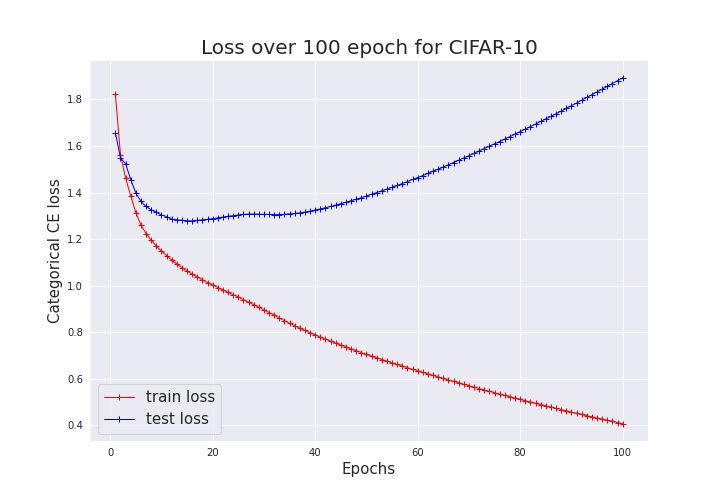
\includegraphics[scale=0.4]{../images/cifar10_100epochs_loss.png}
 \caption{\textit{The image shows a common overfitting behaviour in Deep Learning Applications. The cross entropy loss for the training set keeps a steady descent while the test set loss start increasing.}}  
 \label{cifar-overfit-loss}
\end{figure}

In figure \ref{cifar-overfit-error} is reported the behaviour of the classification error in the same experiment. The trend is 

\begin{figure}[H]
  \centering
  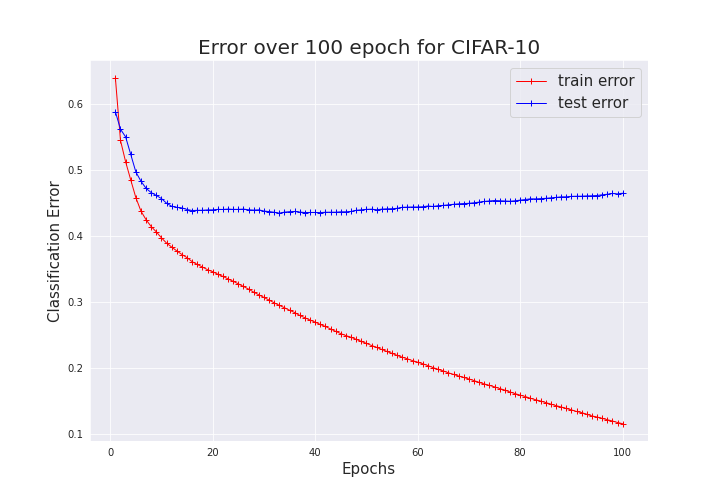
\includegraphics[scale=0.4]{../images/cifar10_100epochs_error.png}
  \caption{\textit{The image shows a common overfitting behaviour in Deep Learning Applications. The classification error in the test set remains almost constant while }}
  \label{cifar-overfit-error}
\end{figure}

The difference in the two graphs is one of the main reasons why accuracy is not a good target function while training deep learning model and, in general, to report machine learning results. Indeed, it only compares a predicted score $t$ to some cutoff $c$, which is not a proper scoring rule and conceals important information about model fitness.
Improper scoring rules such as proportions classified correctly, sensitivity, and specificity are not only arbitrary (in choice of threshold) but are improper, i.e., they have the property that maximizing them leads to a bad model, inaccurate predictions, and selecting the wrong features. 

Cross-entropy loss is more viable than accuracy because it is sensitive to "how wrong" the results are: if the label is $1$, but $t=0.9$, the cross-entropy is lower than when the label is $1$ but $t=0.1$.
The phenomenon when comparing these two graphs - accuracy is flat but loss is increasing - happens because $t>c$.

\section*{Number of Parameters in DL models}

For the current sections, I tested how the number of parameters can influence overfitting in a "simple" dataset such as CIFAR-10. 
The work is inspired by the paper in \cite{Mit-overfit}. 

\section*{Conclusion}


\newpage
\nocite{*}

\bibliographystyle{abbrv}
\bibliography{biblio}


\end{document}
